% [原文 p.49]
\begin{proof}
  这可由引理 2.4.2 与自然同构映射
  \[
  \begin{aligned}
  K(X)&\cong\tilde K(X)\oplus K(y_0)\\
  K(Y)&\cong\tilde K(Y)\oplus K(y_0)
  \end{aligned}
  \]
  立即推出。
\end{proof}

至此，核心命题的准备已经完成。

\begin{proposition*}{2.4.4}
  对 $(X,Y)\in\mathcal{C}^2$，存在自然的（向左无限延伸的）正合列
  \[
  \begin{aligned}
  \cdots\longrightarrow K^{-2}(Y)&\xrightarrow{\ \delta\ }K^{-1}(X,Y)
  \xrightarrow{j^*}K^{-1}(X)\xrightarrow{i^*}K^{-1}(Y)\\
  &\xrightarrow{\ \delta\ }K^0(X,Y)\xrightarrow{j^*}K^0(X)\xrightarrow{i^*}K^0(Y)
  \end{aligned}
  \]
\end{proposition*}

\begin{proof}
  首先注意，只需对 $(X,Y)\in\mathcal{C}^2$ 与 $Y\in\mathcal{C}^+$ 证明 5 项正合列
  \[
  (*)\qquad \tilde K^{-1}(X)\xrightarrow{i^*}\tilde K^{-1}(Y)\xrightarrow{\ \delta\ }K^0(X,Y)
  \xrightarrow{j^*}\tilde K^0(X)\xrightarrow{i^*}\tilde K^0(Y)
  \]
  存在即可。事实上，若能证明这一条，则对 $n=1,2,\ldots$ 把 $(X,Y)$ 换成 $(S^nX,S^nY)$，便得到重复 $(*)$ 的无限序列。再把 $(X,Y)$ 看作 $\mathcal{C}^2$ 的任意对，换成 $(X^+,Y^+)$，就得到所要的无限序列。现在，推论 2.4.3 给出 $(*)$ 右侧 3 项的正合性。为得到剩余部分的正合性，这次把推论 2.4.3 用于对 $(X\cup CY,X)$ 与 $((X\cup CY)\cup CX,\,X\cup CY)$。首先，对 $(X\cup CY,X)$ 得到正合列
  \[
  K(X\cup CY,X)\xrightarrow{m^*}\tilde K(X\cup CY)\xrightarrow{k^*}\tilde K(X)
  \]
  （其中 $k$、$m$ 是自然包含映射）。由于 $CY$ 可缩，由引理 1.4.7 可知映射
% [原文 p.50]
  \[
  p^*\colon\tilde K(X/Y)\longrightarrow\tilde K(X\cup CY)
  \]
  是同构，其中
  \[
  p\colon X\cup CY\longrightarrow X\cup CY/CY=X/Y
  \]
  是把 $CY$ 收缩成一点的映射。又合成 $k^*\circ p^*$ 与 $j^*$ 一致。把映射
  \[
  \theta\colon K(X\cup CY,X)\longrightarrow\tilde K^{-1}(Y)
  \]
  取作引理 2.4.2 之前引入的同构，并由 $\delta=m^*\theta^{-1}$ 定义
  \[
  \delta\colon\tilde K^{-1}(Y)\longrightarrow K(X,Y),
  \]
  便得到正合列
  \[
  \tilde K^{-1}(Y)\xrightarrow{\ \delta\ }K(X,Y)\xrightarrow{j^*}\tilde K(X).
  \]
  这就是 $(*)$ 的中间部分。

  最后，把推论 2.4.3 用于对
  \[
  (X\cup C_1Y\cup C_2X,\;X\cup C_1Y),
  \]
  这里为区别两个锥而把它们命名为 $C_1$、$C_2$（参看下图）。
  \[
  \begin{tikzpicture}[scale=0.85,every node/.style={inner sep=2pt}]
  \coordinate (A) at (0,0);
  \coordinate (M) at (2.6,0);
  \coordinate (P) at (5.4,0);
  \coordinate (T) at (4.0,1.7);
  \coordinate (B) at (2.7,-2.0);
  \draw (A) -- (P);
  \draw (M) -- (T) -- (P);
  \draw (A) -- (B) -- (P);
  \node[above right] at (T) {$C_1Y$};
  \node[below] at (B) {$C_2X$};
  \node[right] at (P) {$X$};
  \node[below] at (3.9,-0.1) {$Y$};
  \end{tikzpicture}
  \]
  于是得到正合列
  \[
  K(X\cup C_1Y\cup C_2X,\,X\cup C_1Y)\longrightarrow
  \tilde K(X\cup C_1Y\cup C_2X)\longrightarrow\tilde K(X\cup C_1Y).
  \]
% [原文 p.51]
  只需再证明这个序列与由 $(*)$ 左侧 3 项得到的序列同构即可。回顾 $\delta$ 的定义便知，只需证明图式
  \[
  \text{(D)}\qquad
  \begin{array}{ccc}
  K(X\cup C_1Y\cup C_2X,\,X\cup C_1Y) & \longrightarrow & \tilde K(X\cup C_1Y\cup C_2X)\\[2pt]
  \Vert & & \Vert\\[2pt]
  \tilde K(C_2X/X) & & \tilde K(C_1Y/Y)\\[2pt]
  \Vert & & \Vert\\[2pt]
  K^{-1}(X) & \xrightarrow{\ i^*\ } & K^{-1}(Y)
  \end{array}
  \]
  除符号的差别之外是可换的。当然，麻烦之处在于：$i^*$ 是由包含映射
  \[
  C_2Y\longrightarrow C_2X
  \]
  诱导的，而图式 (D) 中出现的却是 $C_1Y$ 而不是 $C_2Y$。为处理这一情形，引入 $Y$ 上的二重锥 $C_1Y\cup C_2Y$。
  \[
  \begin{tikzpicture}[scale=0.9]
  \draw (0,0) -- (7.4,0);
  \draw (4.8,0) -- (6.1,1.9) -- (7.4,0) -- (6.1,-1.9) -- cycle;
  \node at (6.1,0.85) {$C_1Y$};
  \node at (6.1,-0.85) {$C_2Y$};
  \end{tikzpicture}
  \]
  它包含在如下的映射交换图式
  \[
  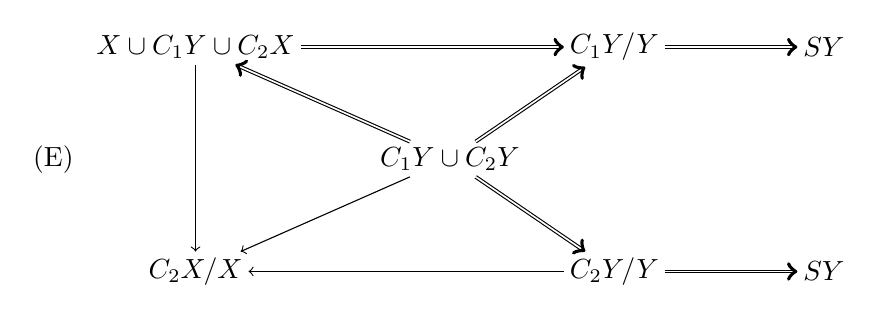
\begin{tikzpicture}[scale=0.95,every node/.style={inner sep=2pt}]
  \node (A) at (0,1.5) {$X\cup C_1Y\cup C_2X$};
  \node (B) at (5.6,1.5) {$C_1Y/Y$};
  \node (C) at (8.4,1.5) {$SY$};
  \node (D) at (3.4,0) {$C_1Y\cup C_2Y$};
  \node (E) at (0,-1.5) {$C_2X/X$};
  \node (F) at (5.6,-1.5) {$C_2Y/Y$};
  \node (G) at (8.4,-1.5) {$SY$};
  \node at (-1.9,0) {(E)};
  \draw[->,double] (A) -- (B);
  \draw[->,double] (B) -- (C);
  \draw[->] (A) -- (E);
  \draw[->,double] (D) -- (A);
  \draw[->,double] (D) -- (B);
  \draw[->] (D) -- (E);
  \draw[->,double] (D) -- (F);
  \draw[->] (F) -- (E);
  \draw[->,double] (F) -- (G);
  \end{tikzpicture}
  \]
  之中。这个图式中所有的双箭头 $\Rightarrow$ 都在 $K$ 中诱导同构映射，因此由 (E) 诱导出的图式
% [原文 p.52]
  \[
  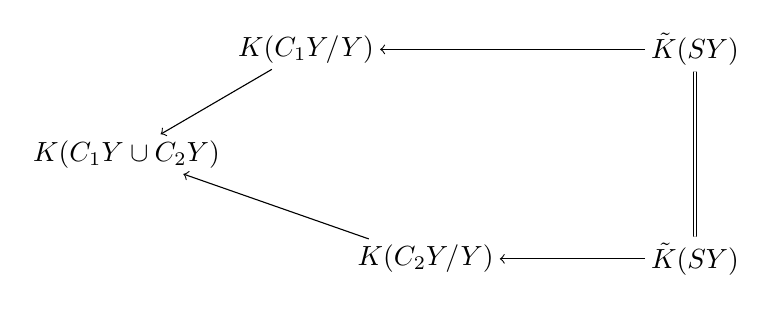
\begin{tikzpicture}[scale=0.95,every node/.style={inner sep=2pt}]
  \node (A) at (2.4,1.4) {$K(C_1Y/Y)$};
  \node (B) at (7.6,1.4) {$\tilde K(SY)$};
  \node (C) at (0,0) {$K(C_1Y\cup C_2Y)$};
  \node (D) at (4.0,-1.4) {$K(C_2Y/Y)$};
  \node (E) at (7.6,-1.4) {$\tilde K(SY)$};
  \draw[->] (B) -- (A);
  \draw[->] (A) -- (C);
  \draw[->] (D) -- (C);
  \draw[->] (E) -- (D);
  \draw[double] (B) -- (E);
  \end{tikzpicture}
  \]
  若除符号之外是可换的，则图式 (D) 也除符号之外可换。这一点可由下面的引理 2.4.5 立即推出。这个引理本身也有独立的意义，后面还要用到。
\end{proof}

% [Tutor Note: 点拨：$\delta$ 定义为 $m^*\theta^{-1}$，先由 $\theta$ 把 $K(X\cup CY,X)$ 送到 $\tilde K^{-1}(Y)$，再用 $m^*$ 拉回。两个映射的顺序不能颠倒，$\delta$ 的符号完全由这个复合决定。]

% [Tutor Note: 点拨：图式 (D) 的左列是锥 $C_2$、右列是锥 $C_1$，交换这两个锥的因子恰好差一个符号；这正是引理 2.4.5 中 $(T\wedge1)^*y=-y$ 的来源，也是作者反复强调“除符号之外”的原因。]

\begin{lemma*}{2.4.5}
  设 $T\colon S^1\to S^1$ 为由 $T(t)=1-t$ $(t\in I)$ 定义的映射（回忆 $S^1=I/\partial I$），并对（$Y\in\mathcal{C}^+$）令 $T\wedge1\colon SY\to SY$ 为由 $S^1$ 上的 $T$ 与 $Y$ 上的恒等映射诱导的映射。此时，对 $y\in\tilde K(SX)$ 有
  \[
  (T\wedge1)^*y=-y.
  \]
\end{lemma*}

% [Tutor Note: 原书 p.52 此处作 $y\in\tilde K(SX)$，与同一陈述中的 $T\wedge1\colon SY\to SY$ 及下文的用法不符，疑为 $\tilde K(SY)$ 之误。正文照原书抄录，请读者按 $SY$ 理解。]

本引理是下一引理的简单推论。

\begin{lemma*}{2.4.6}
  对任意映射 $f\colon Y\to\mathrm{GL}(n,\C)$，记与之对应的 $SY$ 上的向量丛为 $E_f$。此时 $f\mapsto[E_f]-[n]$ 诱导出群同构映射
  \[
  \lim_{n\to\infty}\,[Y,\mathrm{GL}(n,\C)]\cong\tilde K(SY),
  \]
  其中左边的群结构由 $\mathrm{GL}(n,\C)$ 的群结构诱导。
\end{lemma*}

\begin{proof}
  实际上，$\tilde K(SY)$ 上的运算 $(T\wedge1)^*$，通过引理 2.4.6 的同构，对应于把映射 $y\mapsto f(y)$ 换成 $y\mapsto f(y)^{-1}$ 的运算。也就是说，它对应于这个群中的逆元。这样，由引理 2.4.6 得到引理 2.4.5，进而得到命题 2.4.4。因此剩下要做的只是证明引理 2.4.6。现在，由引理 1.4.9，$f\mapsto[E_f]-[n]$ 诱导出集合的双射
  \[
  \lim_{n\to\infty}\,[Y,\mathrm{GL}(n,\C)]\longrightarrow\tilde K(SY).
  \]
  这一双射实际上是群同构，这一事实
% [原文 p.53]
  由连接两个映射
  \[
  (A,B)\longmapsto\begin{pmatrix}A&0\\0&B\end{pmatrix},
  \qquad
  (A,B)\longmapsto\begin{pmatrix}AB&0\\0&1\end{pmatrix}
  \]
  的 $\mathrm{GL}(n)\times\mathrm{GL}(n)\to\mathrm{GL}(2n)$ 的同伦的存在推出。这个同伦具体地由 $0\le t\le\pi/2$ 时的
  \[
  \rho_t(A,B)=
  \begin{pmatrix}A&0\\0&1\end{pmatrix}
  \begin{pmatrix}\cos t&\sin t<本地路径> t&\cos t\end{pmatrix}
  \begin{pmatrix}1&0\\0&B\end{pmatrix}
  \begin{pmatrix}\cos t&-\sin t\\\sin t&\cos t\end{pmatrix}
  \]
  给出。
\end{proof}

由命题 2.4.4 立即得到下面的推论。

\begin{corollary*}{2.4.7}
  若 $Y$ 是 $X$ 的收缩核，则对一切 $n\ge0$，序列
  \[
  K^{-n}(X,Y)\longrightarrow K^{-n}(X)\longrightarrow K^{-n}(Y)
  \]
  是分裂短正合列，并且
  \[
  K^{-n}(X)\cong K^{-n}(X,Y)\oplus K^{-n}(Y)
  \]
  成立。
\end{corollary*}

\begin{corollary*}{2.4.8}
  当 $X$、$Y$ 是带基点的空间时，投影 $\pi_X\colon X\times Y\to X$ 与 $\pi_Y\colon X\times Y\to Y$ 对一切 $n\ge0$ 诱导出同构映射
  \[
  \tilde K^{-n}(X\times Y)\cong\tilde K^{-n}(X\wedge Y)\oplus\tilde K^{-n}(X)\oplus\tilde K^{-n}(Y).
  \]
\end{corollary*}

\begin{proof}
  $X$ 是 $X\times Y$ 的收缩核，而 $Y$ 是 $(X\times Y)/X$ 的收缩核。对此两次应用推论 2.4.7，即得推论的主张。
\end{proof}

由于 $\tilde K^0(X\wedge Y)$ 是 $i_X^*\oplus i_Y^*\colon K^0(X\times Y)\to K^0(X)\oplus K^0(Y)$ 的核，通常的张量积 $K^0(X)\otimes K^0(Y)\to K^0(X\times Y)$ 诱导出积
\[
\tilde K^0(X)\otimes\tilde K^0(Y)\longrightarrow\tilde K^0(X\wedge Y).
\]
% [原文 p.54]
于是得到积
\[
\tilde K^{-n}(X)\otimes\tilde K^{-m}(Y)\longrightarrow\tilde K^{-n-m}(X\wedge Y).
\]
这是因为 $S^nX\wedge S^mY=S^n\wedge S^m\wedge X\wedge Y=S^{n+m}\wedge X\wedge Y$。把 $X$ 换成 $X^+$、把 $Y$ 换成 $Y^+$，便得到积
\[
K^{-n}(X)\otimes K^{-m}(Y)\longrightarrow K^{-n-m}(X\times Y).
\]
用这个积，可以把周期性定理改述如下。

\begin{theorem*}{2.4.9}
  对任意空间 $X$ 与任意 $n\ge0$，映射 $K^{-2}(*)\otimes K^{-n}(X)\to K^{-n-2}(X)$ 诱导出同构映射
  \[
  \beta\colon K^{-n}(X)\longrightarrow K^{-n-2}(X).
  \]
\end{theorem*}

\begin{proof}
  $K^{-2}(*)=\tilde K(S^2)$ 是由 $[H]-[1]$ 生成的自由阿贝尔群。当 $(X,Y)\in\mathcal{C}^2$ 时，命题 2.4.4 的正合列中的映射都与周期性定理的同构映射 $\beta$ 可交换。事实上，这一点对 $i^*$ 与 $j^*$ 成立是容易看出的；而 $\delta$ 由空间之间的映射诱导，故也与 $\beta$ 可交换。
\end{proof}

换言之，$\beta$ 把整个序列向左平移 6 项。其结果是，用 $K^n=K^{n-2}$ 归纳地定义 $n>0$ 时的 $K^n(X,Y)$，就可以把命题 2.4.4 扩充成向两侧无限延伸的正合列。与此等价地，也可以用周期性定理的同构映射 $\beta$ 定义出 6 项正合列
\[
\begin{array}{ccccc}
K^0(X,Y) & \longrightarrow & K^0(X) & \longrightarrow & K^0(Y)\\[6pt]
\uparrow & & & & \downarrow\\[6pt]
K^1(Y) & \longleftarrow & K^1(X) & \longleftarrow & K^1(X,Y)
\end{array}
\]
特别地，除非另作声明，总把 $K^n$ 与 $K^{n-2}$ 视为同一。这里引入
\[
K^*(X)=K^0(X)\oplus K^1(X).
\]
把 $K^*(X,Y)$ 定义为 $K^0(X,Y)\oplus K^1(X,Y)$。此时，对任意一对 $(X,Y)$
% [原文 p.55]
都有正合列
\[
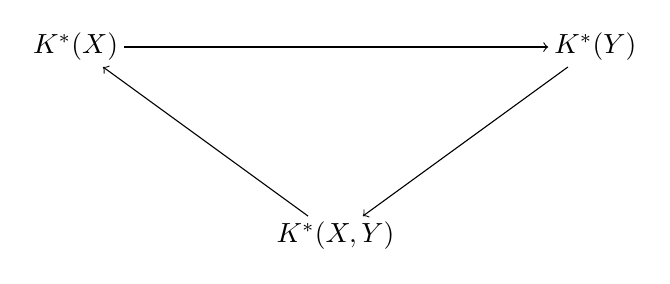
\begin{tikzpicture}[scale=1,every node/.style={inner sep=2pt}]
\node (A) at (0,1.5) {$K^*(X)$};
\node (B) at (6.6,1.5) {$K^*(Y)$};
\node (C) at (3.3,-0.9) {$K^*(X,Y)$};
\draw[->] (A) -- (B);
\draw[->] (C) -- (A);
\draw[->] (B) -- (C);
\end{tikzpicture}
\]

% [Tutor Note: 点拨：6 项正合列画成一个循环，两个竖直箭头都是 $\delta$：右边是 $K^0(Y)\xrightarrow{\delta}K^1(X,Y)$，左边是 $K^1(Y)\xrightarrow{\delta}K^0(X,Y)$。把 $K^n$ 与 $K^{n-2}$ 同一化之后，$\delta$ 才能首尾相接成环。]

定理 2.4.9 的周期性定理是一般的“Thom 同型定理”的特例。$X$ 是紧空间、$E$ 是 $X$ 上的实向量丛时，$E$ 的 Thom 复形 $X^E$ 是 $E$ 的全空间的单点紧化。同样，若 $E$ 是复向量丛，则 $X^E=P(E\oplus1)/P(E)$。由此可见，$\tilde K(X^E)$ 是 $K(X)$ 上的模。下面叙述关于复线丛的 Thom 同型定理。

\begin{theorem*}{2.4.10}
  设 $L$ 为复线丛。则 $\tilde K(X^L)$ 是以一个生成元 $\mu(L)$ 为基的自由 $K(X)$ 模，而 $\mu(L)$ 在 $K(P(L\oplus1))$ 中的像是 $[H]-[L^*]$。
\end{theorem*}

\begin{proof}
  这由决定 $K(P(L\oplus1))$ 的本书主定理以及对 $(P(L\oplus1),P(L))$ 的正合列立即推出（注意 $P(L)=X$）。
\end{proof}

本节最后，把引理 2.4.5 作如下推广。它在后面要用到。

\begin{lemma*}{2.4.11}
  设 $T_\sigma\colon S^nX\to S^nX$ 为由 $S^n=S^1\wedge S^1\wedge\cdots\wedge S^1$ 的 $n$ 个因子的置换 $\sigma$ 诱导的映射。此时，对 $x\in\tilde K(S^nX)$ 有
  \[
  (T_\sigma)^*x=\operatorname{sgn}(\sigma)x.
  \]
\end{lemma*}

\begin{proof}
  把 $S^n$ 看作 $\R^n$ 的单点紧化，就可以让 $\mathrm{GL}(n,\R)$ 作用于它。于是也可以让 $\mathrm{GL}(n,\R)$ 作用于 $\tilde K(S^nX)$。这个作用正是置换作用 $T_\sigma$ 的扩充。$\mathrm{GL}(n,\R)$ 的连通分支只有两个，且由 $\operatorname{sgn}\det$ 刻画，所以只需对某个满足 $\det T=-1$ 的 $T\in\mathrm{GL}(n,\R)$ 验证 $T^*x=-x$。然而，由引理 2.4.5，这个式子
% [原文 p.56]
  对
  \[
  T=\begin{pmatrix}-1&&&\\&1&&\\&&\ddots&\\&&&1\end{pmatrix}
  \]
  成立。
\end{proof}

\section{$K^*(X)$ 的计算}
\takeaway{用周期性定理算出球面的 K 群：$n$ 为奇数时 $\tilde K(S^n)=0$，$n$ 为偶数时 $\tilde K(S^n)=\Z$，由此证明 Brouwer 不动点定理；随后对胞腔复形与射影丛逐一算出 $K^*$，工具是 $K^*(X)=K^0(X)\oplus K^1(X)$ 与分裂正合列。}

由周期性定理可知，$n$ 为奇数时 $\tilde K(S^n)=0$，$n$ 为偶数时 $\tilde K(S^n)=\Z$。用这一点可以证明 Brouwer 不动点定理。

\begin{theorem*}{2.5.1}
  设 $D^n$ 为 $n$ 维欧氏空间的单位圆盘。若 $f\colon D^n\to D^n$ 连续，则存在 $x\in D^n$ 使 $f(x)=x$。
\end{theorem*}

\begin{proof}
  由于 $\tilde K^*(D^n)=0$ 而 $\tilde K^*(S^{n-1})\ne0$，$S^{n-1}$ 不是 $D^n$ 的收缩核。若对一切 $x\in D^n$ 都有 $f(x)\ne x$，则定义 $g\colon D^n\to S^{n-1}$ 为
  \[
  g(x)=(1-\alpha(x))f(x)+\alpha(x)x,
  \]
  其中 $\alpha(x)$ 是满足 $\alpha(x)\ge0$ 与 $|g(x)|=1$ 的唯一函数。若对一切 $x$ 都有 $f(x)\ne x$，这样的函数 $\alpha(x)$ 显然存在。若 $x\in S^{n-1}$，则 $\alpha(x)=1$ 且 $g(x)=x$。于是 $g$ 是 $D^n$ 到 $S^{n-1}$ 上的收缩。
\end{proof}

% [Tutor Note: 点拨：定理 2.5.1 的证明只用到一件事——$S^{n-1}$ 不是 $D^n$ 的收缩核。而这一点由 $\tilde K^*(D^n)=0$、$\tilde K^*(S^{n-1})\ne0$ 得出：收缩核会给出 $K^*$ 上的分裂单射，与两者不同构矛盾。]

空间 $X$ 是胞腔复形，指的是存在由闭集合给出的滤过
\[
X_{-1}\subset X_0\subset X_1\subset\cdots\subset X_n=X,
\]
使 $X_{-1}=\emptyset$，且各 $X_k-X_{k-1}$ 是 $k$ 维开胞腔的不交并。

\begin{proposition*}{2.5.2}
  若 $X$ 是胞腔复形，且对一切 $k$ 都有 $X_{2k}=X_{2k+1}$，则 $K^1(X)=0$，而 $K^0(X)$ 是以与 $X$ 的胞腔一一对应的元素为基的自由阿贝尔群。
\end{proposition*}

\begin{proof}
% [原文 p.57]
  对 $n$ 用归纳法。$X_{2n}/X_{2n-1}$ 是把若干个 $2n$ 维球面在同一点粘合而得，所以以 $k$ 记 $X$ 的 $2n$ 维胞腔的个数时，
  \[
  K^1(X_{2n},X_{2n-2})=0,\qquad K^0(X_{2n},X_{2n-2})=\Z^k
  \]
  成立。于是，关于 $X_{2n}$ 的结论由归纳法假设与对 $(X_{2n},X_{2n-2})$ 的正合列推出。
\end{proof}

% [Tutor Note: 次数约定：命题 2.5.2 中的 $K^1(X)=0$ 依赖把 $K^n$ 与 $K^{n-2}$ 同一化的约定；这里的 $K^1$ 就是奇数次群 $K^{-1}$，不是另一个独立的群。]

能应用这个命题的空间的例子有复 Grassmann 流形、旗流形，以及齐次定义方程形如 $\sum_i z_i^2=0$ 的复二次超曲面。后面将更详细地考察 Grassmann 流形与旗流形。

\begin{proposition*}{2.5.3}
  设 $L_1,\ldots,L_n$ 为 $X$ 上的线丛，$H$ 为 $P(L_1\oplus\cdots\oplus L_n)$ 上的标准线丛。此时，映射 $t\mapsto[H]$ 诱导出 $K(X)$ 模的同构映射
  \[
  K(X)[t]\Big/\prod_{i=1}^{n}\bigl(t-[L_i^*]\bigr)
  \longrightarrow K(P(L_1\oplus\cdots\oplus L_n)).
  \]
\end{proposition*}

\begin{proof}
  先说明可以假定 $L_n=1$。事实上，对 $X$ 上任意向量丛 $E$ 与线丛 $L$，有 $P(E\otimes L)=P(E)$；而 $P(E\otimes L^*)$ 与 $P(E)$ 上的标准线丛 $G$ 与 $H$ 由 $G^*=H^*\otimes L$ 相联系，即 $G=H\otimes L^*$。取 $E=L_1\oplus\cdots\oplus L_n$、$L=L_n^*$，便知关于 $L_1\oplus\cdots\oplus L_n$ 的命题主张与令 $M_i=L_i\otimes L_n^*$ 后关于 $M_1\oplus\cdots\oplus M_n$ 的命题主张等价。因此以下假定 $L_n=1$。为简便起见，记
  \[
  P_m=P(L_1\oplus\cdots\oplus L_m)\qquad(1\le m\le n),
  \]
  则有包含映射 $X=P_1\to P_2\to\cdots\to P_n$。用 $H_m$ 表示 $P_m$ 上的标准线丛，则 $H_m|_{P_{m-1}}\cong H_{m-1}$。此时考虑交换图
% [原文 p.58]
  \[
  \begin{array}{ccc}
  P_{n-1} & \xrightarrow{\ s\ } & P(H_{n-1}^*\oplus1)\\[2pt]
  {\scriptstyle\pi_{n-1}}\big\downarrow & & \big\downarrow{\scriptstyle q}\\[2pt]
  P_1 & \xrightarrow{\ i_n\ } & P_n
  \end{array}
  \]
  （其中 $\pi_{n-1}$ 是到 $X=P_1$ 的投影，$i_n$ 是包含映射，$s$ 是零截面）。它诱导出同胚
  \[
  P(H_{n-1}^*\oplus1)/s(P_{n-1})\longrightarrow P_n/P_1.
  \]
  进一步，$q^*(H_n)$ 与 $P(H_{n-1}^*\oplus1)$ 上的标准线丛 $G$ 同构。又 $K(P(H_{n-1}^*\oplus1))$ 是以两个生成元 $[1]$ 与 $[G]$ 为基的自由 $K(P_{n-1})$ 模，而 $[G]$ 满足等式 $([G]-[1])([G]-[H_{n-1}])=0$。由于 $s^*[G]=[1]$，$K(P(H_{n-1}^*\oplus1),s(P_{n-1}))$ 是由 $[G]-[1]$ 自由生成的子模，且在这个子模上 $[G]$ 与 $[H_{n-1}]$ 的乘法一致。于是，$K(P_n,P_1)$ 是由 $[H_n]-[1]$ 自由生成的自由 $K(P_{n-1})$ 模，其模结构满足：对任意 $x\in K(P_n,P_1)$ 有
  \[
  [H_{n-1}]x=[H_n]x.
  \]
  这里，假定命题对 $n-1$ 成立，则当 $t$ 对应于 $[H_{n-1}]$ 时，
  \[
  K(P_{n-1})\cong K(X)[t]\Big/\prod_{i=1}^{n-1}\bigl(t-[L_i^*]\bigr)
  \]
  是同构。于是可知，$t\mapsto[H_n]$ 诱导出从
  \[
  K(X)[t]\Big/(t-1)\prod_{i=1}^{n-1}\bigl(t-[L_i^*]\bigr)
  \]
  的理想 $(t-1)$ 到 $K(P_n,P_1)$ 上的同构映射。又
  \[
  K(P_n)\cong K(P_n,P_1)\oplus K(X),
  \]
  且 $L_n=1$，所以这个同构映射给出关于 $K(P_n)$ 所要的结果，归纳法成立，证明完成。
\end{proof}

% CHUNK ch02c DONE
